\tikzstyle{reco} = [rectangle,minimum height=4em,text centered, fill=blue!20,draw=black]
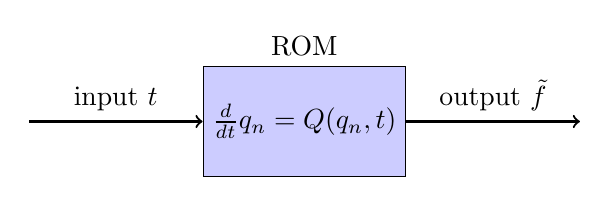
\begin{tikzpicture}[auto]
	\node [reco,label=ROM] (red) {$\frac{d}{dt}q_n = Q(q_n,t)$};
	\draw [<-,thick] (red)--+ (-3.5,0) node[midway,above] {input \(t\)};
	\draw [->,thick] (red)--+ (3.5,0) node[midway,above] {output $\tilde{f}$};
\end{tikzpicture}
